%%%%%%%%%%%%%%%%%%%%%%%%%%%%%%%%%%%%%%%%%%%%%%%%%%%%%%%%%%%%%%%%%%%%%
% Use the koma-script document style
\documentclass{scrbook}
%\KOMAoptions{twoside=false} % disable two-side formatting for scrbook
% alternatively, for shorter essay, use the following
% \documentclass{scrartcl}
%%%%%%%%%%%%%%%%%%%%%%%%%%%%%%%%%%%%%%%%%%%%%%%%%%%%%%%%%%%%%%%%%%%%%

%%%%%%%%%%%%%%%%%%%%%%%%%%%%%%%%%%%%%%%%%%%%%%%%%%%%%%%%%%%%%%%%%%%%%
% Useful packages
\usepackage{mathtools}
\usepackage{amssymb,bm,bbold}
\usepackage{enumerate}

\usepackage{hhline}
\usepackage{float}

% CSCI-265
\usepackage{tikz}
\usetikzlibrary{automata, positioning, arrows}


%=================================
% pre-defined theorem environments
\usepackage{amsthm}
\newtheorem{theorem}{Theorem}
\newtheorem{lemma}{Lemma}
\newtheorem{proposition}{Proposition}
\newtheorem{corollary}{Corollary}
\newtheorem{definition}{Definition}
\newtheorem*{remark}{Remark}
\newtheorem*{assumption}{Assumption}

%=================================
% useful commands
\DeclareMathOperator*{\argmin}{arg\,min}
\DeclareMathOperator*{\argmax}{arg\,max}
\DeclareMathOperator*{\supp}{supp}

\def\vec#1{{\ensuremath{\bm{{#1}}}}}
\def\mat#1{\vec{#1}}

%=================================
% convenient notations
\newcommand{\XX}{\mathbb{X}}
\newcommand{\RR}{\mathbb{R}}
\newcommand{\NN}{\mathbb{N}}
\newcommand{\QQ}{\mathbb{Q}}
\newcommand{\ZZ}{\mathbb{Z}}
\newcommand{\EE}{\mathbb{E}}
\newcommand{\PP}{\mathbb{P}}

\newcommand{\sL}{\mathcal{L}}
\newcommand{\sX}{\mathcal{X}}
\newcommand{\sY}{\mathcal{Y}}

\newcommand{\ind}{\mathbb{1}}

\newcommand{\kleene}{{}^\ast}

%%%%%%%%%%%%%%%%%%%%%%%%%%%%%%%%%%%%%%%%%%%%%%%%%%%%%%%%%%%%%%%%%%%%%
% Typography, change document font
\usepackage[tt=false, type1=true]{libertine}
\usepackage[varqu]{zi4}
\usepackage[libertine]{newtxmath}
\usepackage[T1]{fontenc}

\usepackage[protrusion=true,expansion=true]{microtype}

\author{Guy Matz}

\begin{document}
	
\tikzset{
	->, % makes the edges directed 
%		>='stealth', % makes the arrow heads bold 
	node distance=3cm, % specifies the minimum distance between two nodes. Change if necessary. 
	every state/.style={thick, fill=gray!10}, % sets the properties for each ’state’ node 
	initial text=$ $, % sets the text that appears on the start arrow 
}
	
\title{Title}
% \maketitle

% \tableofcontents
% 
% %\bibliography{bibfile}
% 
% \end{document}


\begin{enumerate}

\item \textbf{Convert the following $\epsilon$-NFA to a DFA:}


  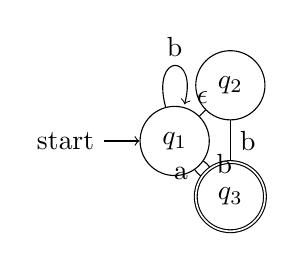
\begin{tikzpicture}
      \node[state, initial] (q1) {$q_1$};
      \node[state,  above right of=q1] (q2) {$q_2$};
      \node[state, accepting, below right of=q1] (q3) {$q_3$};
      \draw
    	(q1) edge[loop above] node{b} (q1)
      (q1) edge[above] node{$\epsilon$} (q2)
      (q2) edge[right] node{b} (q3)

      (q1) edge[bend right=10,  left] node{a} (q3)
      (q3) edge[bend right=10, right] node{b} (q1)
      ;
  \end{tikzpicture}
\\\\

  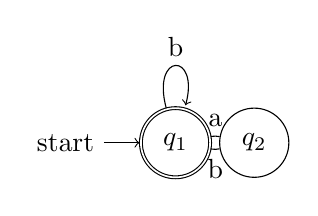
\begin{tikzpicture}
	\node[state, accepting, initial] (q1) {$q_1$};
	\node[state,  right of=q1] (q2) {$q_2$};
	\draw
	(q1) edge[loop above] node{b} (q1)
	
	(q1) edge[bend left=10,  above] node{a} (q2)
	(q2) edge[bend left=10, below] node{b} (q1)
	;
\end{tikzpicture}

\newpage
\item \textbf{Find the regular expression that describes the language accepted by the $\epsilon$-NFA in the question above. Then describe the language in English.}
$$\left( b \kleene \left( ab \right) \kleene \right) \kleene $$
\\
"$ab$"s with any number of "$b$"s

\newpage
\item \textbf{Find the regular expression that describes the language accepted by the following $\epsilon$-NFA}

  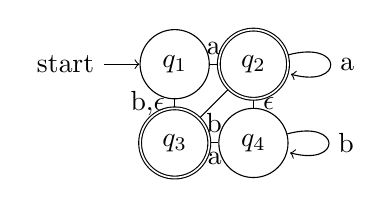
\begin{tikzpicture}
\node[state, initial] (q1) {$q_1$};
\node[state,  accepting, right of=q1] (q2) {$q_2$};
\node[state, accepting,  below of=q1] (q3) {$q_3$};
\node[state, below of=q2] (q4) {$q_4$};
\draw
(q1) edge[above] node{a} (q2)
(q2) edge[loop right] node{a} (q2)
(q3) edge[left] node{b,$\epsilon$} (q1)

(q4) edge[right] node{$\epsilon$} (q2)
(q2) edge[below] node{b} (q3)
(q4) edge[loop right] node{b} (q4)      
(q3) edge[below] node{a} (q4)
      ;
  \end{tikzpicture}

$$ a \left( a\kleene b \left(  \left( a b \kleene \epsilon \right) + \left( b + \epsilon \right) a \right) \right) \kleene $$

\newpage
\item \textbf{Find the union and intersection of the 2 following DFAs:}
\\\\

  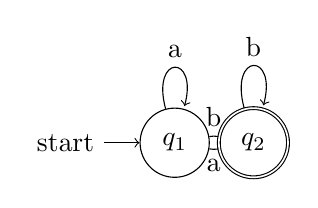
\begin{tikzpicture}
	\node[state, initial] (q1) {$q_1$};
	\node[state,  accepting, right of=q1] (q2) {$q_2$};
	\draw
	(q1) edge[loop above] node{a} (q1)
	
	(q1) edge[bend left=10,  above] node{b} (q2)
	(q2) edge[bend left=10, below] node{a} (q1)
	
	(q2) edge[loop above] node{b} (q2)
	;
\end{tikzpicture}

  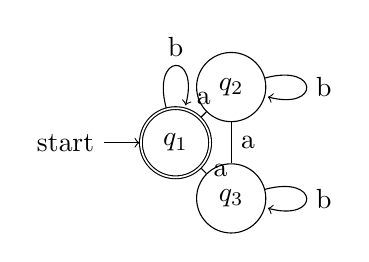
\begin{tikzpicture}
	\node[state, accepting, initial] (q1) {$q_1$};
	\node[state,  above right of=q1] (q2) {$q_2$};
	\node[state, below right of=q1] (q3) {$q_3$};
	\draw
	(q1) edge[loop above] node{b} (q1)
	(q1) edge[above] node{a} (q2)
	(q2) edge[loop right] node{b} (q2)
	(q2) edge[right] node{a} (q3)
	(q3) edge[loop right] node{b} (q3)
	(q3) edge[right] node{a} (q1)
	;
\end{tikzpicture}
\begin{enumerate}
	\item \textbf{Union:}
	
	  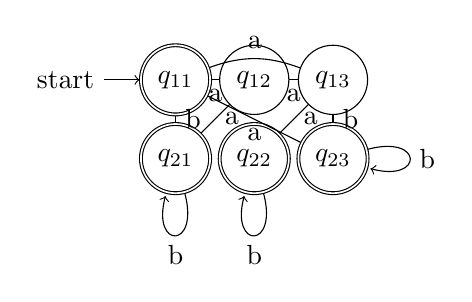
\begin{tikzpicture}
		\node[state, accepting, initial] (q11) {$q_{11}$};
		\node[state,  right of=q11] (q12) {$q_{12}$};
		\node[state,  right of=q12] (q13) {$q_{13}$};
		\node[state, accepting, below of=q11] (q21) {$q_{21}$};
		\node[state,  accepting, right of=q21] (q22) {$q_{22}$};
		\node[state,  accepting, right of=q22] (q23) {$q_{23}$};
		
		\draw
		
		
		(q13) edge[bend right=20,  above] node{a} (q11)
		(q23) edge[bend left=0, below] node{a} (q11)
		
		(q11) edge[bend left=0, below] node{a} (q12)
		(q12) edge[bend left=0, below] node{a} (q13)
		(q13) edge[bend left=0, right] node{b} (q23)
		(q22) edge[bend left=0, right] node{a} (q13)
		(q21) edge[bend left=0, right] node{a} (q12)				
		(q11) edge[bend left=0, right] node{b} (q21)
		
		(q21) edge[loop below] node{b} (q21)
		(q22) edge[loop below] node{b} (q22)
		(q23) edge[loop right] node{b} (q23)
		;
	\end{tikzpicture}
	
	\item \textbf{Intersection:}
	
		  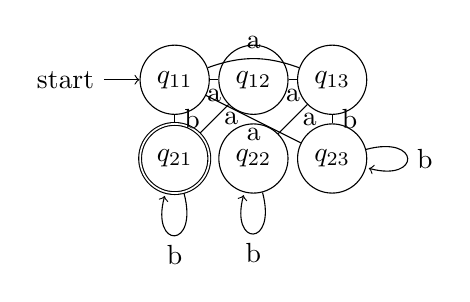
\begin{tikzpicture}
		\node[state, initial] (q11) {$q_{11}$};
		\node[state,  right of=q11] (q12) {$q_{12}$};
		\node[state,  right of=q12] (q13) {$q_{13}$};
		\node[state, accepting, below of=q11] (q21) {$q_{21}$};
		\node[state,  right of=q21] (q22) {$q_{22}$};
		\node[state,  right of=q22] (q23) {$q_{23}$};
		
		\draw
		(q13) edge[bend right=20,  above] node{a} (q11)
		(q23) edge[bend left=0, below] node{a} (q11)
		
		(q11) edge[bend left=0, below] node{a} (q12)
		(q12) edge[bend left=0, below] node{a} (q13)
		(q13) edge[bend left=0, right] node{b} (q23)
		(q22) edge[bend left=0, right] node{a} (q13)
		(q21) edge[bend left=0, right] node{a} (q12)				
		(q11) edge[bend left=0, right] node{b} (q21)
		
		(q21) edge[loop below] node{b} (q21)
		(q22) edge[loop below] node{b} (q22)
		(q23) edge[loop right] node{b} (q23)
		;
	\end{tikzpicture}

\end{enumerate}

\newpage
\item \textbf{Find the DFAs that recognize the complement of each of the original DFAs, respectively, from the previous question}
\\\\
  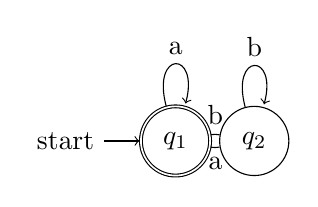
\begin{tikzpicture}
	\node[state, accepting, initial] (q1) {$q_1$};
	\node[state, right of=q1] (q2) {$q_2$};
	\draw
	(q1) edge[loop above] node{a} (q1)
	
	(q1) edge[bend left=10,  above] node{b} (q2)
	(q2) edge[bend left=10, below] node{a} (q1)
	
	(q2) edge[loop above] node{b} (q2)
	;
\end{tikzpicture}

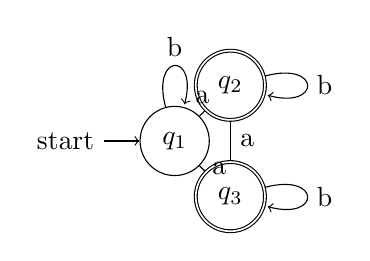
\begin{tikzpicture}
	\node[state, initial] (q1) {$q_1$};
	\node[state,  accepting, above right of=q1] (q2) {$q_2$};
	\node[state, accepting, below right of=q1] (q3) {$q_3$};
	\draw
	(q1) edge[loop above] node{b} (q1)
	(q1) edge[above] node{a} (q2)
	(q2) edge[loop right] node{b} (q2)
	(q2) edge[right] node{a} (q3)
	(q3) edge[loop right] node{b} (q3)
	(q3) edge[right] node{a} (q1)
	;
\end{tikzpicture}

\newpage
\item \textbf{Using the techniques from the last 2 problems, create a DFA that recognizes the language of all words that have an odd number of $a$'s and don't end in $ab$.}
\\\\

\begin{figure}[h]
	\centering
	\caption{Words with an odd Number of $a$'s:}
	  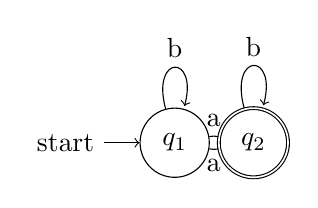
\begin{tikzpicture}
	\node[state, initial] (q1) {$q_1$};
	\node[state, accepting, right of=q1] (q2) {$q_2$};
	\draw
	(q1) edge[loop above] node{b} (q1)
	
	(q1) edge[bend left=10,  above] node{a} (q2)
	(q2) edge[bend left=10, below] node{a} (q1)
	
	(q2) edge[loop above] node{b} (q2)
	;
\end{tikzpicture}
\end{figure}

\begin{figure}[h]
\centering
\caption{Words that end in $ab$}
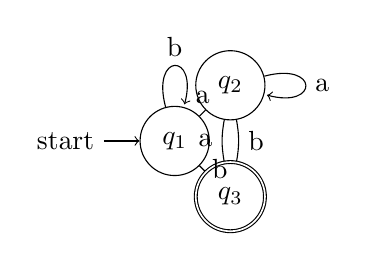
\begin{tikzpicture}[object/.style={thin,double,<->}]
	\node[state, initial] (q1) {$q_1$};
	\node[state, above right of=q1] (q2) {$q_2$};
	\node[state, accepting, below right of=q1] (q3) {$q_3$};
	\draw
	(q1) edge[loop above] node{b} (q1)
	(q1) edge[above] node{a} (q2)
	(q2) edge[loop right] node{a} (q2)
	(q2) edge[bend left=10, right] node{b} (q3)
	(q3) edge[bend left=10, left] node{a} (q2)
	(q3) edge[right] node{b} (q1)
	;
\end{tikzpicture}
	
\end{figure}

\begin{figure}
\centering
\caption{Words that DON'T end in $ab$}
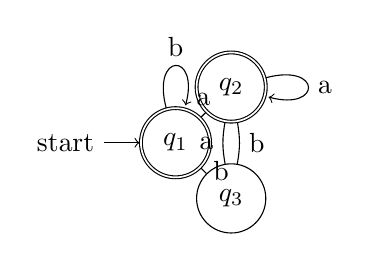
\begin{tikzpicture}
	\node[state, accepting, initial] (q1) {$q_1$};
	\node[state,  accepting, above right of=q1] (q2) {$q_2$};
	\node[state, below right of=q1] (q3) {$q_3$};
	\draw
	(q1) edge[loop above] node{b} (q1)
	(q1) edge[above] node{a} (q2)
	(q2) edge[loop right] node{a} (q2)
	(q2) edge[bend left=10, right] node{b} (q3)
	(q3) edge[bend left=10, left] node{a} (q2)
	(q3) edge[right] node{b} (q1)
	;
\end{tikzpicture}
\end{figure}

\begin{figure}
	\centering
	\caption{Words that have an odd number of $a$'s and don't end in $ab$\\(Intersection of Figures 1 \& 3 above)}
	\begin{tikzpicture}
		\node[state, initial] (q11) {$q_{11}$};
		\node[state, right of=q11] (q12) {$q_{12}$};
		\node[state, right of=q12] (q13) {$q_{13}$};
		\node[state, accepting, below of=q11] (q2) {$q_{21}$};
		\node[state,  accepting, right of=q21] (q22) {$q_{22}$};
		\node[state, right of=q22] (q23) {$q_{23}$};
		
		\draw
		(q11) edge[loop above] node{b} (q11)
		(q21) edge[loop below] node{b} (q21)
		(q11) edge[right] node{a} (q22)
		(q12) edge[above] node{b} (q13)
		(q12) edge[bend left=10, right] node{a} (q22)
		(q13) edge[bend right=20, above] node{b} (q11)
		(q13) edge[ right] node{a} (q22)
		(q21) edge[below] node{a} (q12)
		(q22) edge[bend left=10, left] node{a} (q12)
		(q22) edge[above] node{b} (q23)
		(q23) edge[ below] node{a} (q12)
		(q23) edge[bend left=20, below] node{b} (q21)
		;
	\end{tikzpicture}
\end{figure}

\newpage
\item \textbf{Do textbook problems 2.3.1, 2.4.1, 2.5.1.}
\\ For 2.3.1 and 2.5.1, the transition tables are just a different way of representing the FA. The algorithm is the same.
2.4.1 asks you go convert the sets of strings to NFAs, not $\epsilon$-NFAs. So while you can easily write regular expressions for them, you can't then use Thompson's Construction exactly -  but you can use the same ideas.
\begin{enumerate}
	\item \textbf{Convert the following NFA to a DFA}
	\begin{table}[H]
						\centering
		\begin{tabular}{c||c|c}
			 &  0 &  1   \\ \hline
			p& $\{p,q\}$ &  $\{p\}$   \\ \hline
			q&  $\{r\}$& $\{r\}$   \\ \hline
			r&  $\{s\}$& $\emptyset$   \\ \hline
			$\kleene s$& $\{s\}$ & $\{s\}$ \\ \hline
		\end{tabular}
	\end{table}

\begin{figure}[h]
	\centering
	%\caption{Words with an odd Number of $a$'s:}
	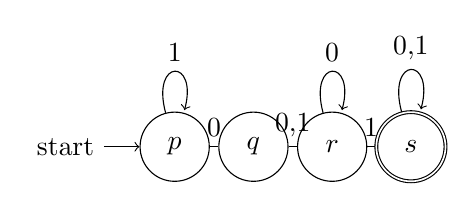
\begin{tikzpicture}
		\node[state, initial] (p) {$p$};
		\node[state, right of=p] (q) {$q$};
		\node[state, right of=q] (r) {$r$};
		\node[state, accepting, right of=r] (s) {$s$};
		\draw
		(p) edge[loop above] node{1} (p)
		
		(p) edge[above] node{0} (q)
		(q) edge[above] node{0,1} (r)
		(r) edge[above] node{1} (s)
		(r) edge[loop above] node{0} (r)
		(s) edge[loop above] node{0,1} (s)
		;		
	\end{tikzpicture}
\end{figure}

	\item \textbf{Design NFA's to to recognize the following sets of strings}
		\begin{enumerate}
			\item abc, abd,and aacd 
				\begin{table}[H]
				\centering
				\begin{tabular}{c||c|c|c|c}
					&  a &  b & c & d \\ \hline
					p& $\{p,q\}$ &  $\emptyset$ & $\emptyset$ & $\emptyset$   \\ \hline
					q&  $\emptyset$ & $\{r\}$& $\emptyset$ &  $\{r\}$   \\ \hline
					r&  $\emptyset$&  $\emptyset$ & $\{s\}$& $\{s\}$  \\ \hline
					$\kleene s$& $\{s\}$ & $\{s\}$ & $\{s\}$ & $\{s\}$ \\ \hline
				\end{tabular}
			\end{table}
		
			\item 0101, 101, and 011
			\\ I'm not sure I understand what to do here
			\item ab, bc, and ca 
		\end{enumerate}

	\item \textbf{Consider the following $\epsilon$-NFA}

		\begin{table}[H]
				\centering
		\begin{tabular}{c||c|c|c|c}
			&  $\epsilon$ &  a   & b & c\\ \hline
			p&  $\emptyset$ &  $\{p\}$  & $\{q\}$& $\{r\}$ \\ \hline
			q&  $\{p\}$& $\{q\}$   & $\{r\}$ &  $\emptyset$\\ \hline
			$\kleene r$&  $\{q\}$& $\{r\}$ &  $\emptyset$ & $\{p\}$ \\ \hline
		\end{tabular}
	\end{table}

			\begin{enumerate}
		\item abc, abd,and aacd 
					\\ I'm not sure I understand what to do here
		\item 0101, 101, and 011
		\item ab, bc, and ca 
	\end{enumerate}
\end{enumerate}

\end{enumerate}

\input{footer.tex}
